\section{Expirement Offline Pipeline}

\subsection{Data Preprocessing}

\subsubsection{Converting the Data from CSV to Parquet}

The raw AliCCP dataset is stored in CSV format. However, to leverage GPU-accelerated libraries such as cuDF, the data is converted into the Apache Parquet \cite{ApacheParquet}.


The original data in CSV format was about 11GB in size. After converting it to Parquet format, the data size was reduced to 1.1GB.
The training data consists of 42,299,771 rows, while the testing data consists of 42,999,775 rows.

\subsubsection{Eliminating Rows with Excessive Missing Data}

Rows with more than five null features were removed to ensure data completeness.
This resulted in a training dataset with 33,088,764 rows and a testing dataset with 33,678,677 rows.

\subsubsection{Resplitting Data}

Originally the data was split with a 1:1 ratio into training and testing data.
To balance the training and testing data, 60\% of the testing data was moved to the training data. 
The resulting datasets contain 53,299,746 training rows and 13,467,695 testing rows.
The ratio of the training data to the testing data is approximately 80:20.


The following table shows the changes made to the data during the preprocessing phase:

\begin{table}[ht]
\centering
\begin{tabular}{|c|c|c|c|}
\hline
\textbf{Data Set} & \textbf{Original Rows} & \textbf{Data After Cleaning} & \textbf{Data After Resplitting} \\
\hline
Training Data & 42,299,771 & 33,088,764 & 53,299,746 \\
\hline
Testing Data & 42,999,775 & 33,678,677 & 13,467,695 \\
\hline
\end{tabular}
\caption{Data Rows Before and After Preprocessing}
\label{tab:data-reprocessing}
\end{table}

\subsubsection{Saving customer and products parquets}

In this step, the user features as well as the item features are extracted from the training data and saved as parquet files.
Those files will later be used as an offline data store by Feast, the feature store that will be used at inference time.

Before saving the parquet files, timestamps are added to the data to help Feast keep track of the data freshness and do incremental materialization.

\subsection{Retrieval Stage}

As mentioned earlier, the retrieval model consists of two towers, the user tower and the item tower. 
The user tower is responsible for processing the user features, while the item tower is responsible for processing the item features.

\subsubsection{Retrieval Model Training}

The model is trained using the following hyperparameters:

\begin{itemize}
\item Batch Size: 28K
\item Number of Epochs: 20
\item Optimizer: Adam
\item Loss Function: Categorical Crossentropy
\item Model: Two Tower 
\end{itemize}

Figure \ref{fig:RetrievalModelTraining} shows the training loss and recall of the retrieval model.
It shows that the model achieves a recall at 20 of around 30\% on the training data, but on the validation data, the recall is around 4\% only.

This means that in the top 20 recommendations, 4\% of the actual positive items in the validation set are listed.
In production, not only 20 but the top hundreds of items are taken from the retrieval model and are fed into the ranking model. 

So if the recall is 4\% at 20, it is expected to be much higher at values like 500 which is used in this project.
Unfortunately, due to technical limitations, the recall at 500 could not be calculated for each user of the dataset.

\begin{figure}[H]
    \centering
    \begin{subfigure}{.5\textwidth}
        \centering
        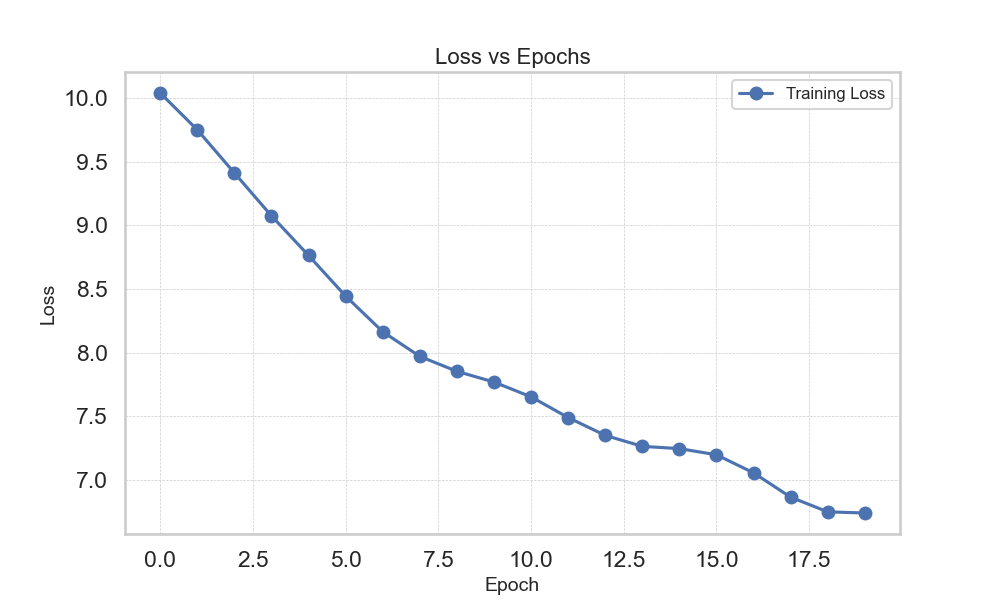
\includegraphics[width=0.95\linewidth]{assets/training_loss.png}
        \caption[Retrieval Model Loss]{Retrieval Model Loss}
        \label{fig:RetrievalModelLoss}
    \end{subfigure}%
    \begin{subfigure}{.5\textwidth}
        \centering
        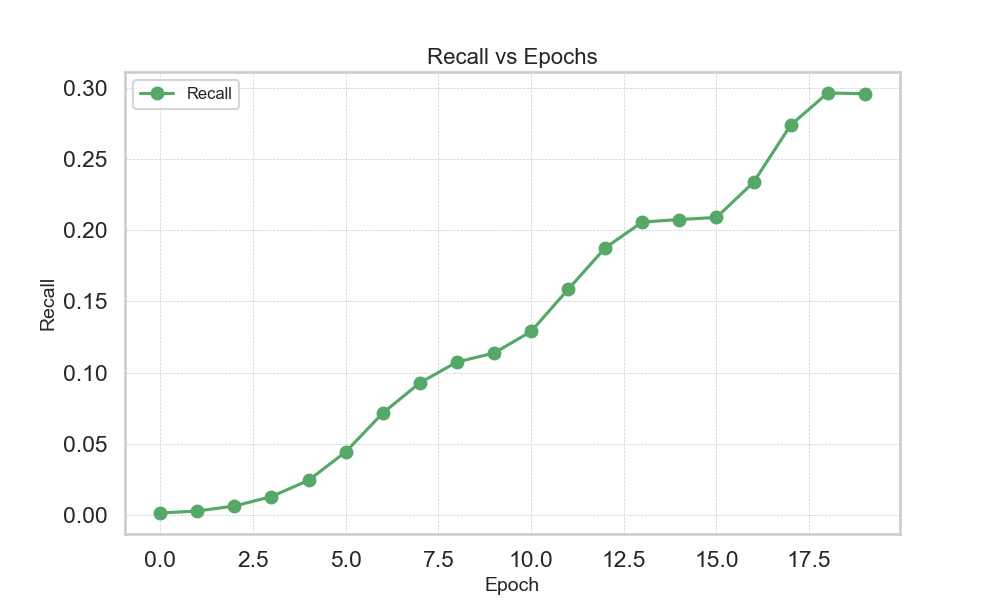
\includegraphics[width=0.95\linewidth]{assets/recall_epochs.png}
        \caption[Retrieval Model Recall]{Retrieval Model Recall At 20}
        \label{fig:RetrievalModelRecall}
    \end{subfigure}
    \caption[Retrieval Model Training]{Retrieval Model Training Results}
    \label{fig:RetrievalModelTraining}
\end{figure}

\subsubsection{Saving Query Tower}

Once the retrieval model is trained, the query tower is saved as a Keras model to the model repository, 
in this project, it should be an S3 bucket, but for the simplicity of this experiment, it is saved locally to a GP3 SSD attached to the server.
This model will be used to generate the user embeddings at inference time.

\subsubsection{Saving Item Embeddings}

the embeddings of each item in the dataset are calculated at training time using the trained retrieval model. 
Then those embeddings are saved in a parquet \cite{ApacheParquet} file which will next be converted to a Faiss \cite{Faiss} index for fast retrieval at inference time.

Once the retrieval model finishes generating the item embedding parquet,
the parquet is used to generate a Faiss \cite{Faiss} index.
In this experiment, the index is saved to the model repository and later loaded to GPU memory on inference server start up.

\subsection{Ranking Model Training}

A DLRM model is trained using the following hyperparameters:

\begin{itemize}
\item Batch Size: 204800
\item Number of Epochs: 2
\item Optimizer: Adam
\end{itemize}

TODO graphs and overfitting !!

Once the model is trained, the model is saved as a Keras model to the model repository.